\chapter{Simple Linear Programming Problems}
When both the objective and all the constraints in Expression \ref{eqn:GeneralMax} are linear functions, then the optimization problem is called a \textit{linear programming problem}. This has the general form:
\begin{equation}
\left\{
\begin{aligned}
\max\;\;& z(x_1,\dots,x_n) = c_1x_1 + \dots + c_nx_n\\
s.t.\;\;& a_{11}x_1 + \dots + a_{1n}x_n \leq b_1\\
& \hspace*{0.5in}\vdots\\
& a_{m1}x_1 + \dots + a_{mn} x_n \leq b_m\\
& h_{11}x_1 + \dots + h_{n1}x_n = r_1\\
&\hspace*{0.5in}\vdots\\
&h_{l1}x_1 + \dots + h_{ln}x_n = r_l
\end{aligned}
\right.
\label{eqn:GeneralLPMax}
\end{equation}

\begin{definition}[Linear Function] A function $z:\mathbb{R}^n \rightarrow \mathbb{R}$ is \textit{linear} if there are constants $c_1,\dots,c_n \in \mathbb{R}$ so that:
\begin{equation}
z(x_1,\dots,x_n) = c_1x_1 + \dots + c_nx_n
\end{equation}
\label{def:LinearFunc}
\end{definition}

\begin{lemma}[Linear Function] If $z:\mathbb{R}^n \rightarrow \mathbb{R}$ is \textit{linear} then for all $\mathbf{x}_1, \mathbf{x}_2 \in \mathbb{R}^n$ and for all scalar constants $\alpha \in \mathbb{R}$ we have:
\begin{gather}
z(\mathbf{x}_1 + \mathbf{x}_2) = z(\mathbf{x}_1) + z(\mathbf{x}_2)\\
z(\alpha \mathbf{x}_1) = \alpha z(\mathbf{x}_1)
\end{gather}
\label{lem:LinearFunc}
\end{lemma}

\begin{exercise} Prove Lemma \ref{lem:LinearFunc}.
\end{exercise}

For the time being, we will eschew the general form and focus exclusively on linear programming problems with two variables. Using this limited case, we will develop a graphical method for identifying optimal solutions, which we will generalize later to problems with arbitrary numbers of variables. 

\begin{example} Consider the problem of a toy company that produces toy planes and toy boats. The toy company can sell its planes for $\$10$ and its boats for $\$8$ dollars. It costs $\$3$ in raw materials to make a plane and $\$2$ in raw materials to make a boat. A plane requires $3$ hours to make and $1$ hour to finish while a boat requires $1$ hour to make and $2$ hours to finish. The toy company knows it will not sell anymore than $35$ planes per week. Further, given the number of workers, the company cannot spend anymore than $160$ hours per week finishing toys and $120$ hours per week making toys. The company wishes to maximize the profit it makes by choosing how much of each toy to produce. 

We can represent the profit maximization problem of the company as a linear programming problem. Let $x_1$ be the number of planes the company will produce and let $x_2$ be the number of boats the company will produce. The profit for each plane is $\$10 - \$3 = \$7$ per plane and the profit for each boat is $\$8 - \$2 = \$6$ per boat. Thus the total profit the company will make is:
\begin{equation}
z(x_1,x_2) = 7x_1 + 6x_2
\end{equation}
The company can spend no more than $120$ hours per week making toys and since a plane takes $3$ hours to make and a boat takes $1$ hour to make we have:
\begin{equation}
3x_1 + x_2 \leq 120
\end{equation}
Likewise, the company can spend no more than $160$ hours per week finishing toys and since it takes $1$ hour to finish a plane and $2$ hour to finish a boat we have:
\begin{equation}
x_1 + 2x_2 \leq 160
\end{equation}
Finally, we know that $x_1 \leq 35$, since the company will make no more than $35$ planes per week. Thus the complete linear programming problem is given as:
\begin{equation}
\left\{
\begin{aligned}
\max\;\;& z(x_1,x_2) = 7x_1 + 6x_2\\
s.t.\;\;&  3x_1 + x_2 \leq 120\\
& x_1 + 2x_2 \leq 160\\
& x_1 \leq 35\\
& x_1 \geq 0\\
& x_2 \geq 0
\end{aligned}
\right.
\label{eqn:ToyMakerEx}
\end{equation}
\label{ex:ToyMaker}
\end{example}

\begin{exercise} A chemical manufacturer produces three chemicals: A, B and C. These chemical are produced by two processes: 1 and 2. Running process 1 for 1 hour costs \$4 and yields 3 units of chemical A, 1 unit of chemical B and 1 unit of chemical C. Running process 2 for 1 hour costs \$1 and produces 1 units of chemical A, and 1 unit of chemical B (but none of Chemical C). To meet customer demand, at least 10 units of chemical A, 5 units of chemical B and 3 units of chemical C must be produced daily. Assume that the chemical manufacturer wants to minimize the cost of production. Develop a linear programming problem describing the constraints and objectives of the chemical manufacturer. [Hint: Let $x_1$ be the amount of time Process 1 is executed and let $x_2$ be amount of time Process 2 is executed. Use the coefficients above to express the cost of running Process 1 for $x_1$ time and Process 2 for $x_2$ time. Do the same to compute the amount of chemicals A, B, and C that are produced.]
\label{exer:ChemicalPlant}
\end{exercise}

\section{Modeling Assumptions in Linear Programming}
Inspecting Example \ref{ex:ToyMaker} (or the more general Problem \ref{eqn:GeneralLPMax}) we can see there are several assumptions that must be satisfied when using a linear programming model. We enumerate these below:
\begin{description}
\item[Proportionality Assumption] A problem can be phrased as a linear program only if the contribution to the objective function \textit{and} the left-hand-side of each constraint by each decision variable $(x_1,\dots,x_n)$ is proportional to the value of the decision variable.

\item[Additivity Assumption] A problem can be phrased as a linear programming problem only if the contribution to the objective function \textit{and} the left-hand-side of each constraint by any decision variable $x_i$ ($i=1,\dots,n$) is completely independent of any other decision variable $x_j$ ($j \neq i$) and additive. 

\item[Divisibility Assumption] A problem can be phrased as a linear programming problem only if the quantities represented by each decision variable are infinitely divisible (i.e., fractional answers make sense). 

\item[Certainty Assumption] A problem can be phrased as a linear programming problem only if the coefficients in the objective function and constraints are known with certainty. 
\end{description}

The first two assumptions simply assert (in English) that both the objective function and functions on the left-hand-side of the (in)equalities in the constraints are linear functions of the variables $x_1,\dots,x_n$. 

The third assumption asserts that a valid optimal answer could contain fractional values for decision variables. It's important to understand how this assumption comes into play--even in the toy making example. Many quantities can be divided into non-integer values (ounces, pounds etc.) but many other quantities cannot be divided. For instance, can we really expect that it's reasonable to make $1/2$ a plane in the toy making example? When values must be constrained to true integer values, the linear programming problem is called an \textit{integer programming problem}. These problems are outside the scope of this course, but there is a \textit{vast} literature dealing with them \cite{PS98,WN99}. For many problems, particularly when the values of the decision variables may become large, a fractional optimal answer could be obtained and then rounded to the nearest integer to obtain a reasonable answer. For example, if our toy problem were re-written so that the optimal answer was to make $1045.3$ planes, then we could round down to $1045$.

The final assumption asserts that the coefficients (e.g., profit per plane or boat) is known with absolute certainty. In traditional linear programming, there is no lack of knowledge about the make up of the objective function, the coefficients in the left-hand-side of the constraints or the bounds on the right-hand-sides of the constraints. There is a literature on \textit{stochastic programming} \cite{KW94,BN02} that relaxes some of these assumptions, but this too is outside the scope of the course.

\begin{exercise} In a short sentence or two, discuss whether the problem given in Example \ref{ex:ToyMaker} meets all of the assumptions of a scenario that can be  modeled by a linear programming problem. Do the same for Exercise \ref{exer:ChemicalPlant}. [Hint: Can you make $2/3$ of a toy? Can you run a process for $1/3$ of an hour?]
\end{exercise}

\begin{exercise} Suppose the costs are not known with certainty but instead a probability distribution for each value of $c_i$ ($i=1,\dots,n$) is known. Suggest a way of constructing a linear program from the probability distributions. [Hint: Suppose I tell you that I'll give you a uniformly random amount of money between $\$1$ and $\$2$. How much money do you expect to receive? Use the same reasoning to answer the question.]
\end{exercise}

\section{Graphically Solving Linear Programs Problems with Two Variables (Bounded Case)}
Linear Programs (LP's) with two variables can be solved graphically by plotting the feasible region along with the level curves of the objective function. We will show that we can find a point in the feasible region that maximizes the objective function using the level curves of the objective function. We illustrate the method first using the problem from Example \ref{ex:ToyMaker}.

\begin{example}[Continuation of Example \ref{ex:ToyMaker}] Let's continue the example of the Toy Maker begin in Example \ref{ex:ToyMaker}. To solve the linear programming problem graphically, begin by drawing the feasible region. This is shown in the blue shaded region of Figure \ref{fig:ToyExampleFeasibleRegion}. 
\begin{figure}[htbp] 
\centering
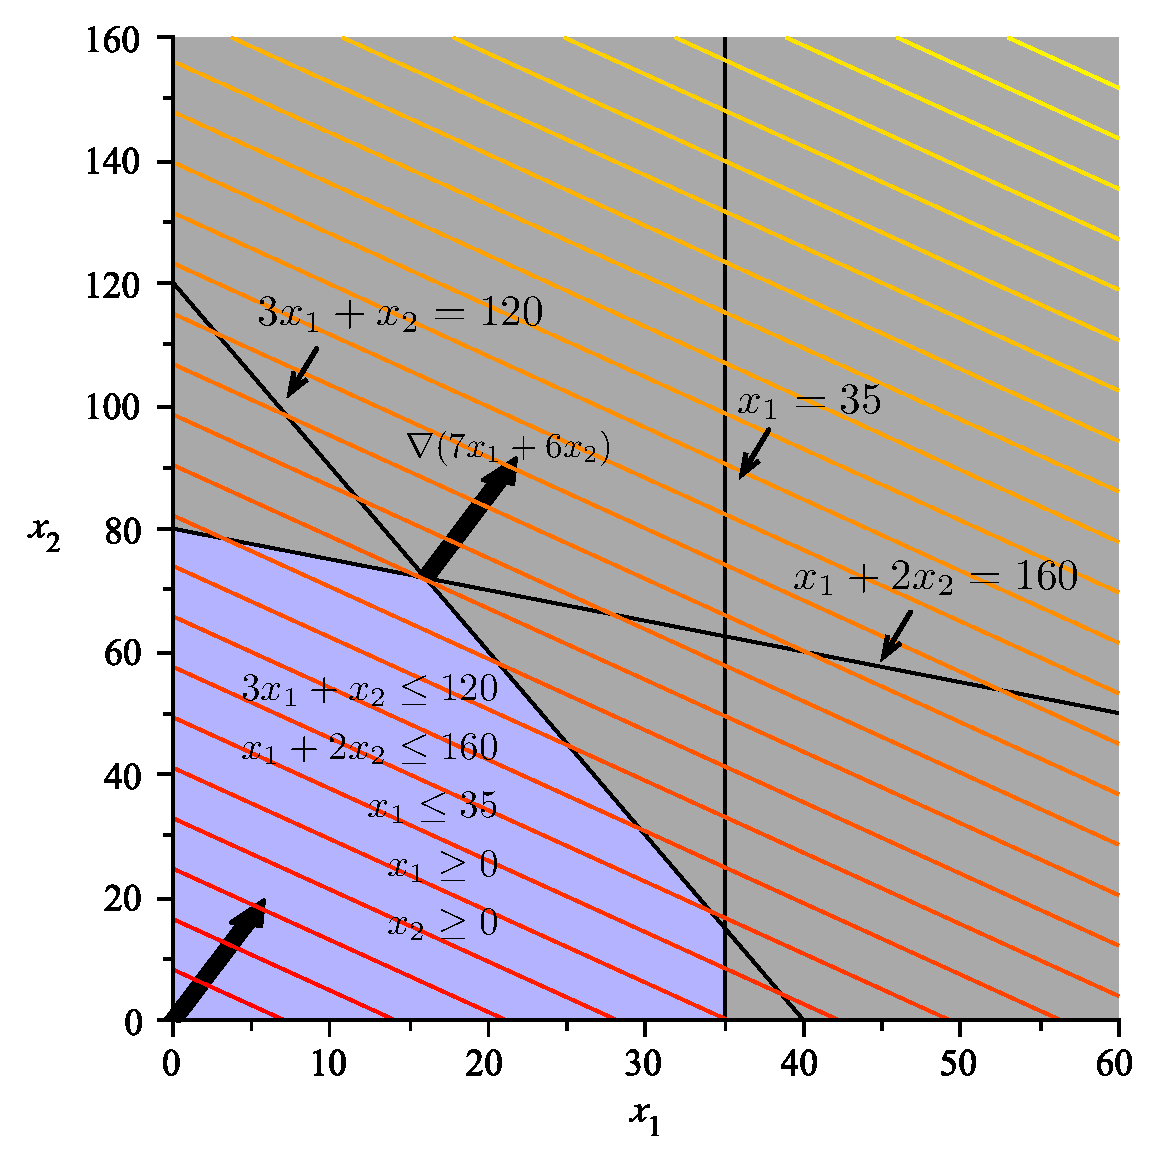
\includegraphics[scale=0.4]{FeasibleRegion.pdf}
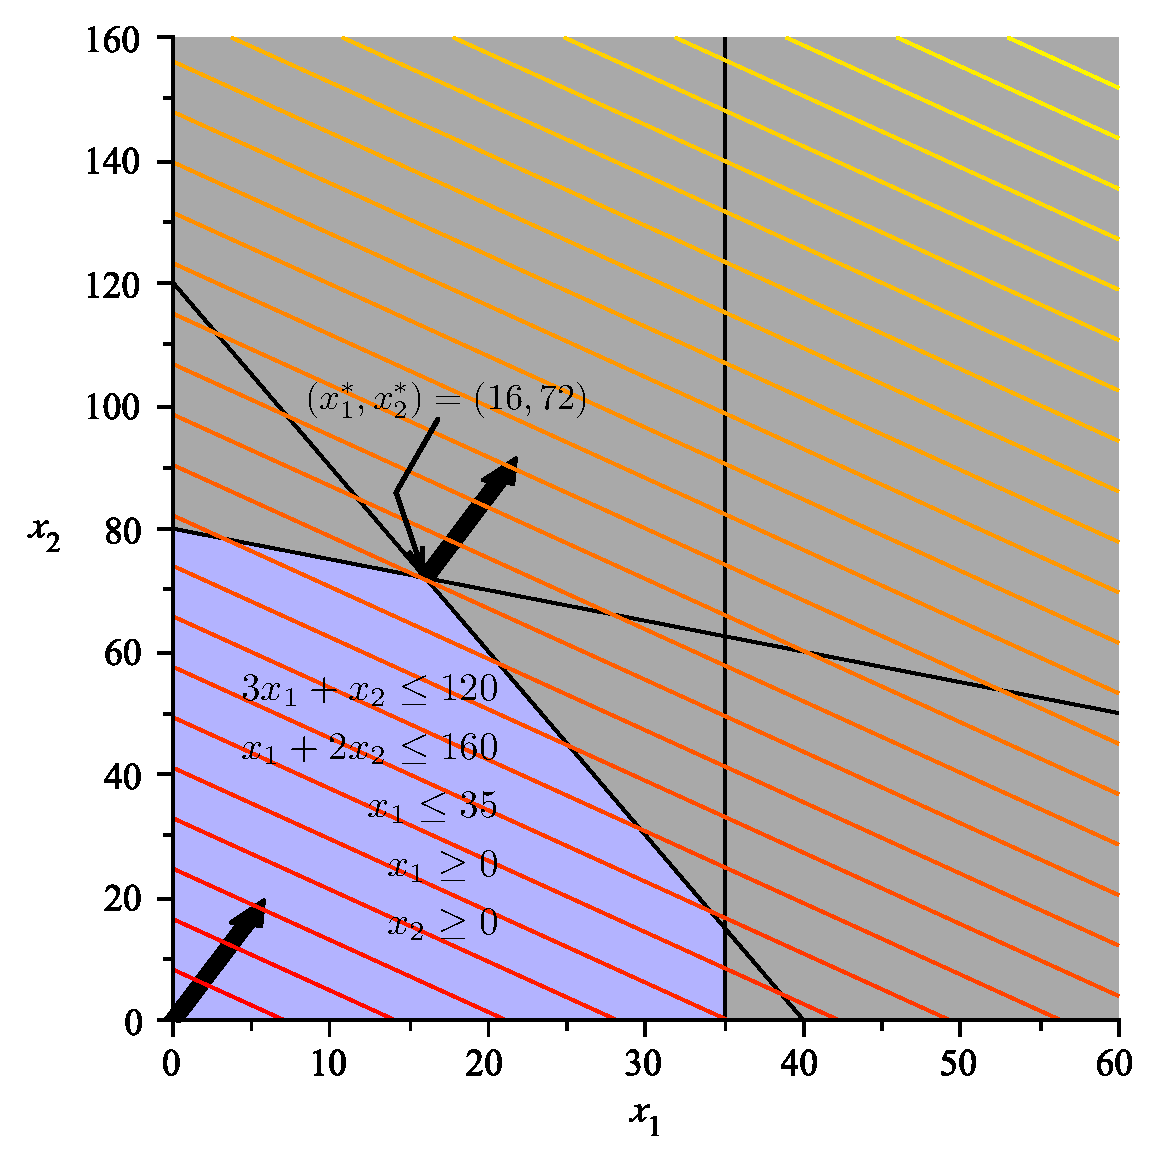
\includegraphics[scale=0.4]{FeasibleRegionWithMax.pdf}
\caption{Feasible Region and Level Curves of the Objective Function: The shaded region in the plot is the feasible region and represents the intersection of the five inequalities constraining the values of $x_1$ and $x_2$. On the right, we see the optimal solution is the ``last'' point in the feasible region that intersects a level set as we move in the direction of increasing profit.}
\label{fig:ToyExampleFeasibleRegion}
\end{figure}

After plotting the feasible region, the next step is to plot the level curves of the objective function. In our problem, the level sets will have the form:
\begin{displaymath}
7x_1 + 6x_2 = c \implies x_2 = \frac{-7}{6}x_1 + \frac{c}{6}
\end{displaymath}
This is a set of parallel lines with slope $-7/6$ and intercept $c/6$ where $c$ can be varied as needed. The level curves for various values of $c$ are parallel lines. In Figure \ref{fig:ToyExampleFeasibleRegion} they are shown in colors ranging from red to yellow depending upon the value of $c$. Larger values of $c$ are more yellow. 

To solve the linear programming problem, follow the level sets along the gradient (shown as the black arrow) until the last level set (line) intersects the feasible region. If you are doing this by hand, you can draw a single line of the form $7x_1 + 6x_2 = c$ and then simply draw parallel lines in the direction of the gradient $(7,6)$. At some point, these lines will fail to intersect the feasible region. The last line to intersect the feasible region will do so at a point that maximizes the profit. In this case, the point that maximizes $z(x_1,x_2) = 7x_1 + 6x_2$, subject to the constraints given, is $(x_1^*, x_2^*) = (16,72)$. 

Note the point of optimality $(x_1^*, x_2^*) = (16,72)$ is at a corner of the feasible region. This corner is formed by the intersection of the two lines: $3x_1 + x_2 = 120$ and $x_1 + 2x_2 = 160$. In this case, the constraints 
\begin{gather*}
3x_1 + x_2 \leq 120\\
x_1 + 2x_2 \leq 160
\end{gather*}
are both \textit{binding}, while the other constraints are non-binding. In general, we will see that when an optimal solution to a linear programming problem exists, it will always be at the intersection of several binding constraints; that is, it will occur at a corner of a higher-dimensional polyhedron.  
\end{example}

\section{Formalizing The Graphical  Method}
In order to formalize the method we've shown above, we will require a few new definitions. 

\begin{definition} Let $r \in \mathbb{R}$, $r \geq 0$ be a non-negative scalar and let $\mathbf{x}_0 \in \mathbb{R}^n$ be a point in $\mathbb{R}^n$. Then the set:
\begin{equation}
B_r(\mathbf{x}_0) = \left\{\mathbf{x} \in \mathbb{R}^n | \;\; ||\mathbf{x} - \mathbf{x}_0|| \leq r\right\}
\end{equation}
is called the \textit{closed ball of radius $r$ centered at point $\mathbf{x}_0$ in $\mathbb{R}^n$}. 
\label{defn:ClosedBall}
\end{definition}
In $\mathbb{R}^2$, a closed ball is just a disk and its circular boundary centered at $\mathbf{x}_0$ with radius $r$. In $\mathbb{R}^3$, a closed ball is a solid sphere and its spherical centered at $\mathbf{x}_0$ with radius $r$. Beyond three dimensions, it becomes difficult to visualize what a closed ball looks like. 

We can use a closed ball to define the notion of boundedness of a feasible region: 
\begin{definition} Let $S \subseteq \mathbb{R}^n$. Then the set $S$ is \textit{bounded} if there exists an $\mathbf{x}_0 \in \mathbb{R}^n$ and finite $r \geq 0$ such that $S$ is totally contained in $B_r(\mathbf{x}_0)$; that is, $S \subset B_r(\mathbf{x}_0)$.
\label{defn:BoundedSet}
\end{definition}
Definition \ref{defn:BoundedSet} is illustrated in Figure \ref{fig:BoundedSet}. The set $S$ is shown in blue while the ball of radius $r$ centered at $\mathbf{x}_0$ is shown in gray. 
\begin{figure}[htbp]
\centering
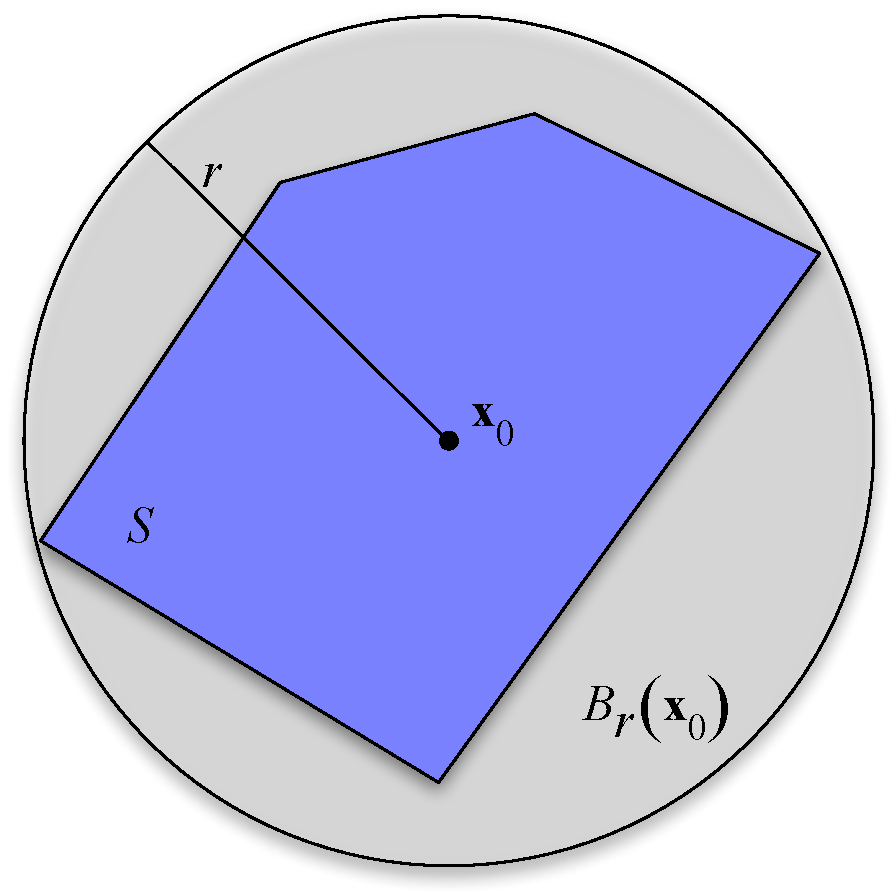
\includegraphics[scale=0.4]{BallBounded.pdf}
\caption{A Bounded Set: The set $S$ (in blue) is bounded because it can be entirely contained inside a ball of a finite radius $r$ and centered at some point $\mathbf{x}_0$. In this example, the set $S$ is in $\mathbb{R}^2$. This figure also illustrates the fact that a ball in $\mathbb{R}^2$ is just a disk and its boundary.}
\label{fig:BoundedSet}
\end{figure}

We can now define an algorithm for identifying the solution to a linear programing problem in two variables with a \textit{bounded} feasible region (see Algorithm \ref{alg:GraphLPBoundedUniqueSoln}): 
\begin{algorithm}
\caption{Algorithm for Solving a Two Variable Linear Programming Problem Graphically--Bounded Feasible Region, Unique Solution Case}
\label{alg:GraphLPBoundedUniqueSoln}
\begin{center}
\begin{minipage}[t]{\textwidth-1em}
\underline{\textbf{Algorithm for Solving a Linear Programming Problem Graphically}}\\
\textit{Bounded Feasible Region, Unique Solution}
\begin{enumerate*}
\item Plot the feasible region defined by the constraints.
\item Plot the level sets of the objective function.
\item For a maximization problem, identify the level set corresponding the greatest (least, for minimization) objective function value that intersects the feasible region. This point will be at a corner. 
\item The point on the corner intersecting the greatest (least) level set is a solution to the linear programming problem.  
\end{enumerate*}
\end{minipage}
\end{center}
\end{algorithm}

The example linear programming problem presented in the previous section has a single optimal solution. In general, the following outcomes can occur in solving a linear programming problem: 
\begin{enumerate*}
\item The linear programming problem has a unique solution. (We've already seen this.)
\item There are infinitely many alternative optimal solutions.
\item There is no solution and the problem's objective function can grow to positive infinity for maximization problems (or negative infinity for minimization problems). 
\item There is no solution to the problem at all. 
\end{enumerate*}

Case 3 above can only occur when the feasible region is unbounded; that is, it cannot be surrounded by a ball with finite radius. We will illustrate each of these possible outcomes in the next four sections. We will prove that this is true in a later chapter.

\begin{exercise} Use the graphical method for solving linear programming problems to solve the linear programming problem you defined in Exercise \ref{exer:ChemicalPlant}.
\end{exercise}

\section{Problems with Alternative Optimal Solutions}
We'll study a specific linear programming problem with an infinite number of solutions by modifying the objective function in Example \ref{ex:ToyMaker}. 
\begin{example}
Suppose the toy maker in Example \ref{ex:ToyMaker} finds that it can sell planes for a profit of $\$18$ each instead of $\$7$ each. The new linear programming problem becomes:
\begin{equation}
\left\{
\begin{aligned}
\max\;\;& z(x_1,x_2) = 18x_1 + 6x_2\\
s.t.\;\;&  3x_1 + x_2 \leq 120\\
& x_1 + 2x_2 \leq 160\\
& x_1 \leq 35\\
& x_1 \geq 0\\
& x_2 \geq 0
\end{aligned}
\right.
\label{eqn:ToyMakerAltOptSoln}
\end{equation}
Applying our graphical method for finding optimal solutions to linear programming problems yields the plot shown in Figure \ref{fig:ToyMakerAltOptSoln}. The level curves for the function $z(x_1,x_2) = 18x_1 + 6x_2$ are \textit{parallel} to one face of the polygon boundary of the feasible region. Hence, as we move further up and to the right in the direction of the gradient (corresponding to larger and larger values of $z(x_1, x_2)$) we see that there is not \textit{one} point on the boundary of the feasible region that intersects that level set with greatest value, but instead a side of the polygon boundary described by the line $3x_1 + x_2 = 120$ where $x_1 \in [16, 35]$. Let:
\begin{displaymath}
S = \{(x_1,x_2) | 3x_1 + x_2 \leq 120,\,x_1 + 2x_2 \leq 160,\,x_1 \leq 35,\,x_1,x_2 \geq 0\}
\end{displaymath} 
that is, $S$ is the feasible region of the problem. Then for any value of $x_1^* \in [16,35]$ and any value $x_2^*$ so that  $3x_1^* + x_2^* = 120$, we will have $z(x_1^*, x_2^*) \geq z(x_1, x_2)$ for all $(x_1,x_2) \in S$. Since there are infinitely many values that $x_1$ and $x_2$  may take on, we see this problem has an infinite number of alternative optimal solutions.
\begin{figure}[htbp]
\centering
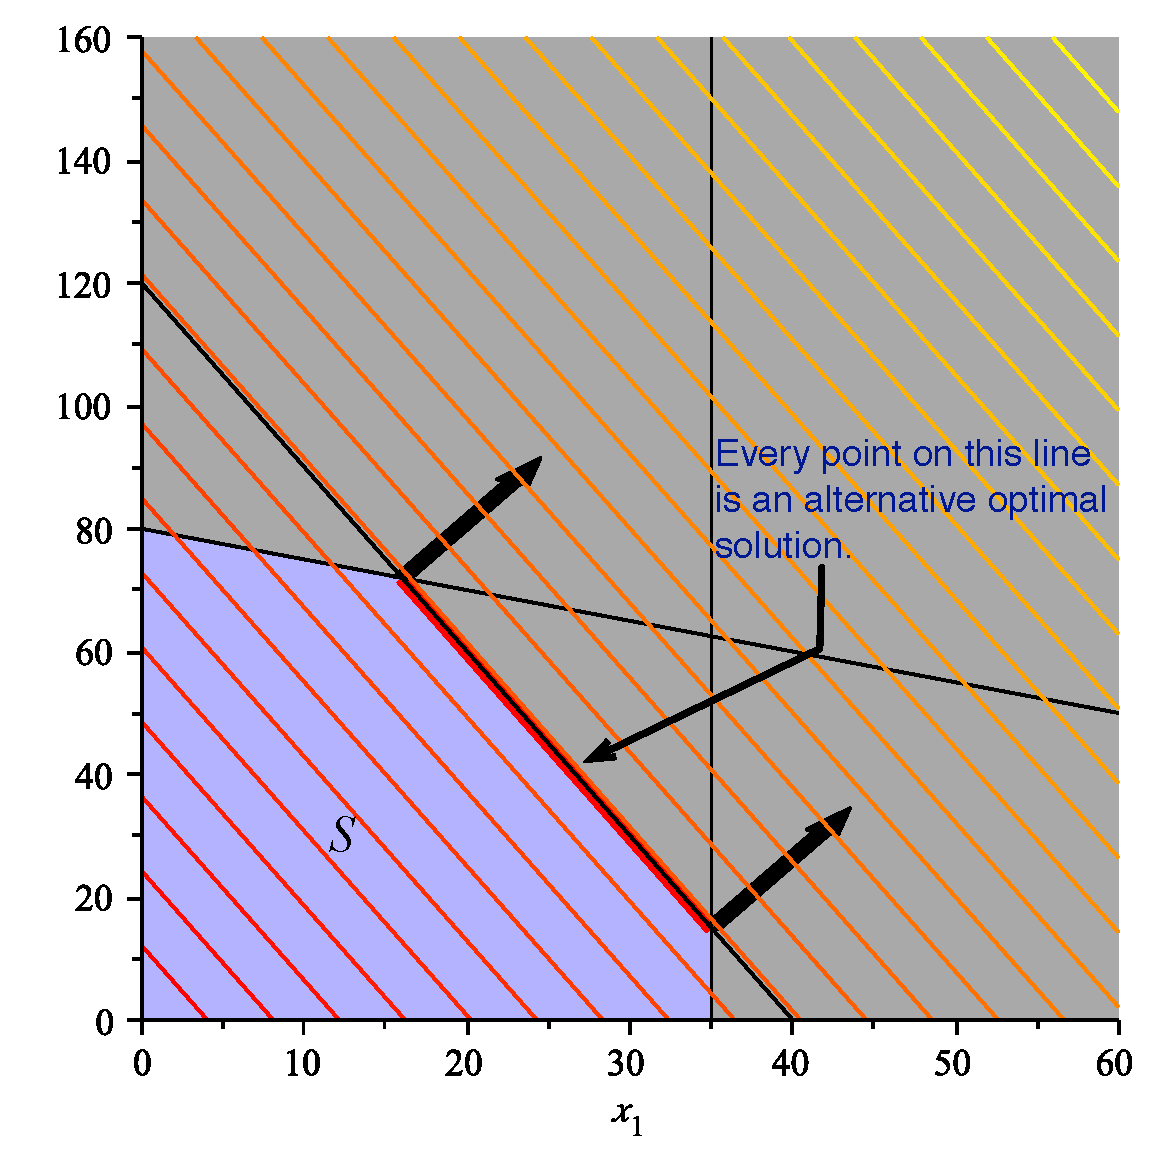
\includegraphics[scale=0.4]{AltOptSolns.pdf}
\caption{An example of infinitely many alternative optimal solutions in a linear programming problem. The level curves for $z(x_1,x_2) = 18x_1 + 6x_2$ are \textit{parallel} to one face of the polygon boundary of the feasible region. Moreover, this side contains the points of greatest value for $z(x_1,x_2)$ inside the feasible region. Any combination of $(x_1,x_2)$ on the line $3x_1 + x_2 = 120$ for $x_1 \in [16, 35]$ will provide the largest possible value $z(x_1,x_2)$ can take in the feasible region $S$.}
\label{fig:ToyMakerAltOptSoln}
\end{figure}
\label{ex:ToyMakerAltOptSoln}
\end{example}

Based on the example in this section, we can modify our algorithm for finding the solution to a linear programming problem graphically to deal with situations with an infinite set of alternative optimal solutions (see Algorithm \ref{alg:GraphLPBounded}):
\begin{algorithm}
\caption{Algorithm for Solving a Two Variable Linear Programming Problem Graphically--Bounded Feasible Region Case}
\label{alg:GraphLPBounded}
\begin{center}
\begin{minipage}[t]{\textwidth-1em}
\underline{\textbf{Algorithm for Solving a Linear Programming Problem Graphically}}\\
\textit{Bounded Feasible Region}
\begin{enumerate*}
\item Plot the feasible region defined by the constraints.
\item Plot the level sets of the objective function.
\item For a maximization problem, identify the level set corresponding the greatest (least, for minimization) objective function value that intersects the feasible region. This point will be at a corner. 
\item The point on the corner intersecting the greatest (least) level set is a solution to the linear programming problem. 
\item \textbf{If the level set corresponding to the greatest (least) objective function value is parallel to a side of the polygon boundary next to the corner identified, then there are infinitely many alternative optimal solutions and any point on this side may be chosen as an optimal solution.} 
\end{enumerate*}
\end{minipage}
\end{center}
\end{algorithm}

\begin{exercise} Modify the linear programming problem from Exercise \ref{exer:ChemicalPlant} to obtain a linear programming problem with an infinite number of alternative optimal solutions. Solve the new problem and obtain a description for the set of alternative optimal solutions. [Hint: Just as in the example, $x_1$ will be bound between two value corresponding to a side of the polygon. Find those values and the constraint that is binding. This will provide you with a description of the form for any $x_1^* \in [a,b]$ and $x_2^*$ is chosen so that $cx_1^* + dx_2^* = v$, the point $(x_1^*, x_2^*)$ is an alternative optimal solution to the problem. Now you fill in values for $a$, $b$, $c$, $d$ and $v$.]
\end{exercise}

\section{Problems with No Solution} Recall for \textit{any} mathematical programming problem, the feasible set or region is simply a subset of $\mathbb{R}^n$. If this region is empty, then there is no solution to the mathematical programming problem and the problem is said to be \textit{over constrained}. We illustrate this case for linear programming problems with the following example.
\begin{example} Consider the following linear programming problem:
\begin{equation}
\left\{
\begin{aligned}
\max\;\;& z(x_1,x_2) = 3x_1 + 2x_2\\
s.t.\;\;&  \frac{1}{40}x_1 + \frac{1}{60}x_2 \leq 1\\
& \frac{1}{50}x_1 + \frac{1}{50}x_2 \leq 1\\
& x_1 \geq 30\\
& x_2 \geq 20
\end{aligned}
\right.
\label{eqn:LPInfeasible}
\end{equation}
The level sets of the objective and the constraints are shown in Figure \ref{fig:LPInfeasible}. 
\begin{figure}[htbp]
\centering
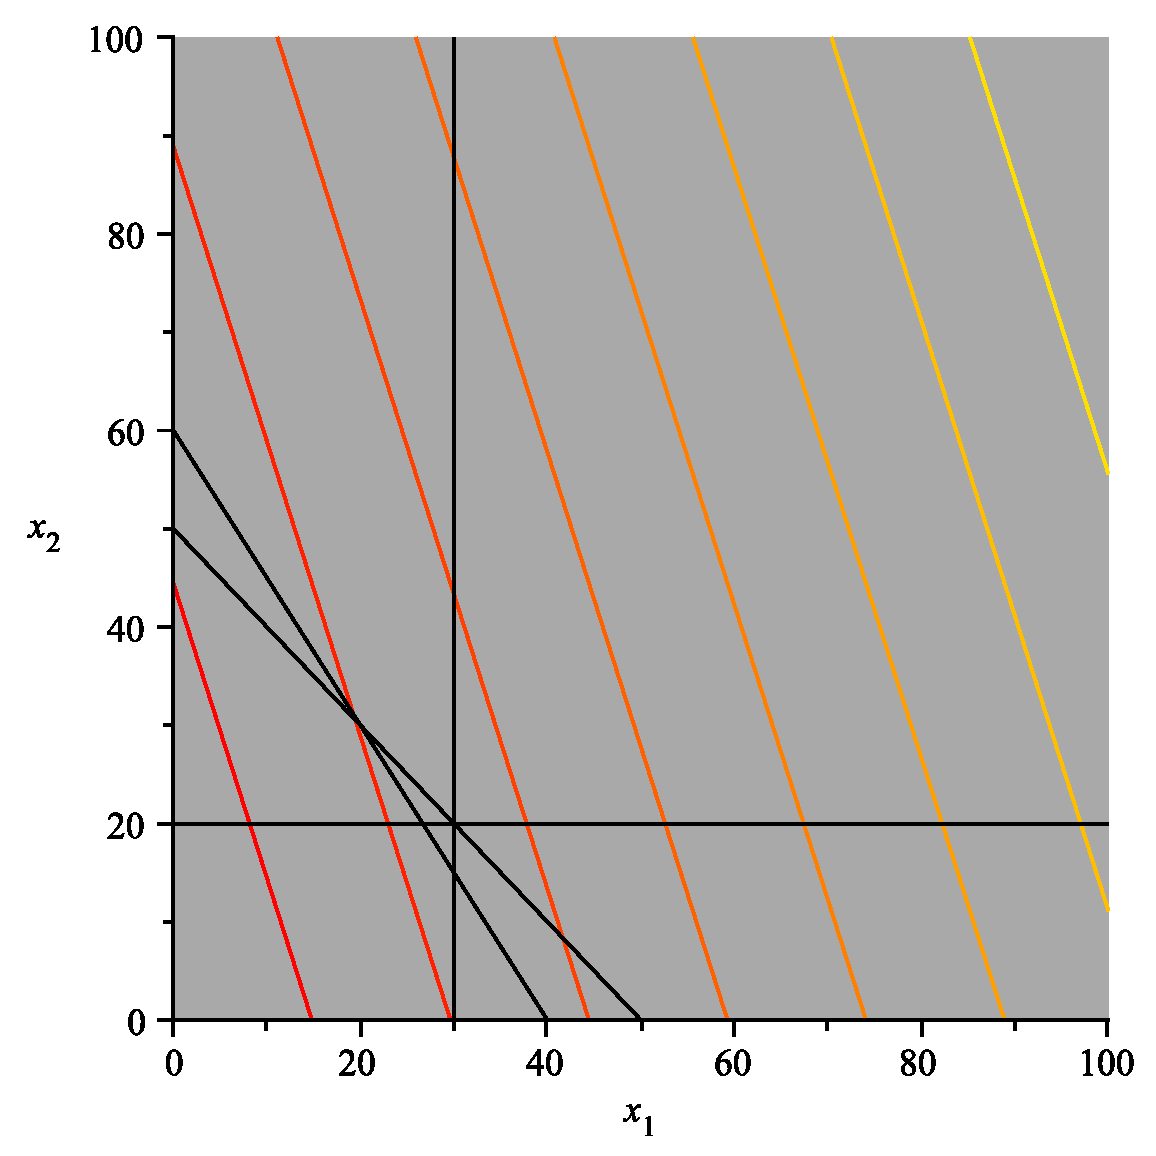
\includegraphics[scale=0.4]{LPNoSoln.pdf}
\caption{A Linear Programming Problem with no solution. The feasible region of the linear programming problem is empty; that is, there are no values for $x_1$ and $x_2$ that can simultaneously satisfy all the constraints. Thus, no solution exists.}
\label{fig:LPInfeasible}
\end{figure}

The fact that the feasible region is empty is shown by the fact that in Figure \ref{fig:LPInfeasible} there is no blue region--i.e., all the regions are gray indicating that the constraints are not satisfiable.
\label{ex:LPNoSoln}
\end{example} 
Based on this example, we can modify our previous algorithm for finding the solution to linear programming problems graphically (see Algorithm \ref{alg:GraphLPBoundedEmpty}):
\begin{algorithm}
\caption{Algorithm for Solving a Two Variable Linear Programming Problem Graphically--Bounded Feasible Region Case}
\label{alg:GraphLPBoundedEmpty}
\begin{center}
\begin{minipage}[t]{\textwidth-1em}
\underline{\textbf{Algorithm for Solving a Linear Programming Problem Graphically}}\\
\textit{Bounded Feasible Region}
\begin{enumerate*}
\item Plot the feasible region defined by the constraints.
\item \textbf{If the feasible region is empty, then no solution exists.}
\item Plot the level sets of the objective function.
\item For a maximization problem, identify the level set corresponding the greatest (least, for minimization) objective function value that intersects the feasible region. This point will be at a corner. 
\item The point on the corner intersecting the greatest (least) level set is a solution to the linear programming problem. 
\item \textbf{If the level set corresponding to the greatest (least) objective function value is parallel to a side of the polygon boundary next to the corner identified, then there are infinitely many alternative optimal solutions and any point on this side may be chosen as an optimal solution.} 
\end{enumerate*}
\end{minipage}
\end{center}
\end{algorithm}

\section{Problems with Unbounded Feasible Regions}
Again, we'll tackle the issue of linear programming problems with unbounded feasible regions by illustrating the possible outcomes using examples.

\begin{example} Consider the linear programming problem below:
\begin{equation}
\left\{
\begin{aligned}
\max\;\;& z(x_1,x_2) = 2x_1 - x_2\\
s.t.\;\;& x_1 - x_2 \leq 1\\
& 2x_1 + x_2 \geq 6\\
&x_1,x_2 \geq 0
\end{aligned}
\right.
\label{eqn:LPUnboundFeasibleRegion1}
\end{equation}
The feasible region and level curves of the objective function are shown in Figure \ref{fig:LPUnboundFeasibleRegion1}. 
\begin{figure}[htbp]
\centering
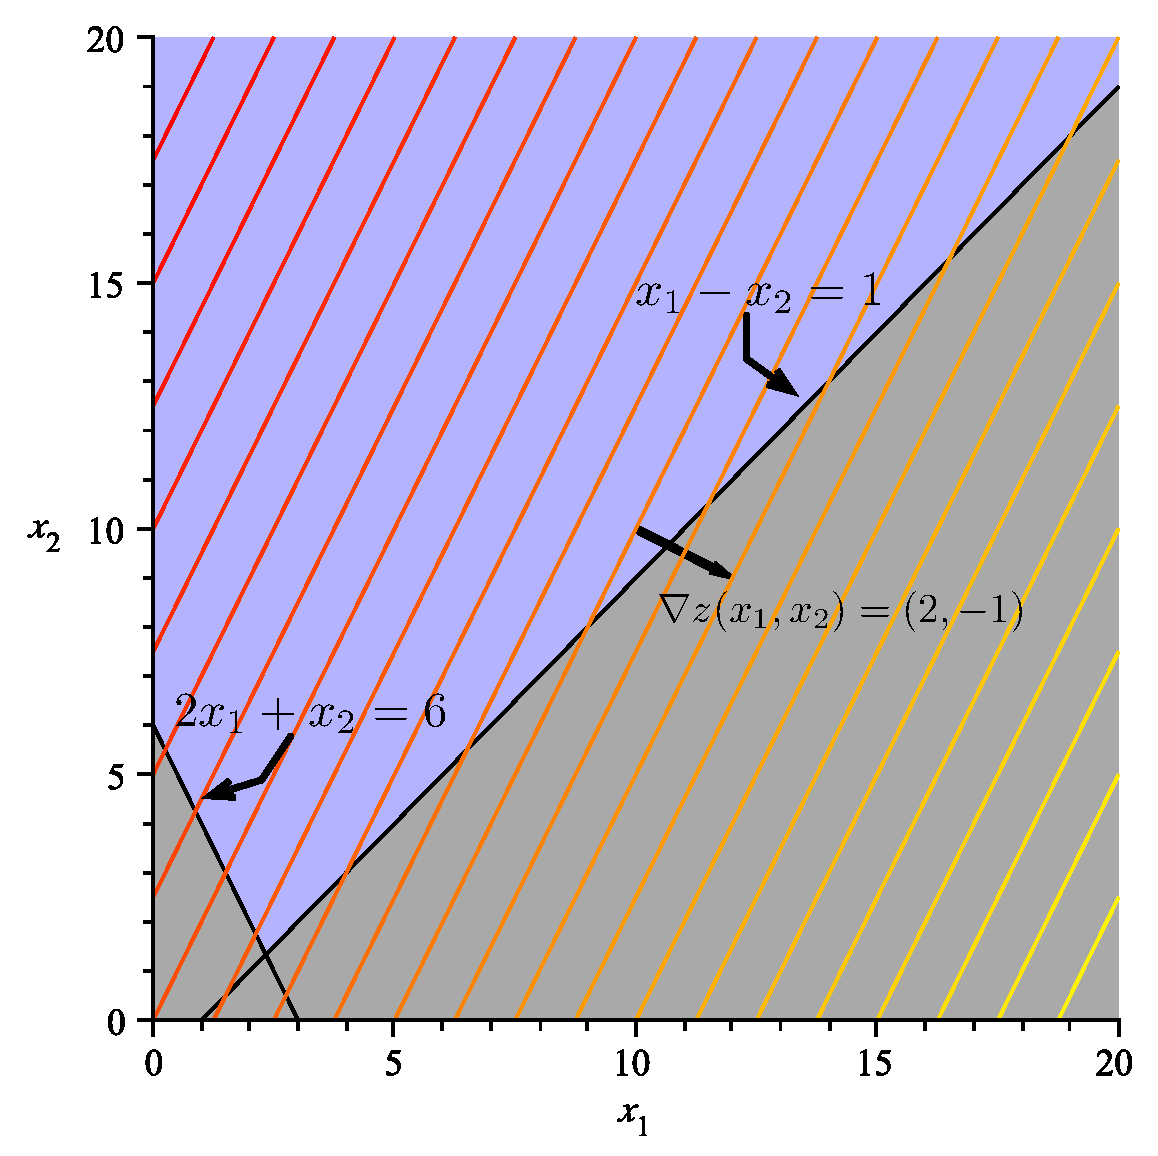
\includegraphics[scale=0.4]{UnboundedFeasibleRegion.pdf}
\caption{A Linear Programming Problem with Unbounded Feasible Region: Note that we can continue to make level curves of $z(x_1,x_2)$ corresponding to larger and larger values as we move down and to the right. These curves will continue to intersect the feasible region for any value of $v = z(x_1,x_2)$ we choose. Thus, we can make $z(x_1,x_2)$ as large as we want and still find a point in the feasible region that will provide this value. Hence, the optimal value of $z(x_1,x_2)$ subject to the constraints $+\infty$. That is, the problem is unbounded.}
\label{fig:LPUnboundFeasibleRegion1}
\end{figure}
The feasible region in Figure \ref{fig:LPUnboundFeasibleRegion1} is clearly unbounded since it stretches upward along the $x_2$ axis infinitely far and also stretches rightward along the $x_1$ axis infinitely far, bounded below by the line $x_1-x_2 = 1$. There is no way to enclose this region by a disk of finite radius, hence the feasible region is not bounded. 

We can draw more level curves of $z(x_1,x_2)$  in the direction of increase (down and to the right) as long as we wish. There will always be an intersection point with the feasible region because it is infinite. That is, these curves will continue to intersect the feasible region for any value of $v = z(x_1,x_2)$ we choose. Thus, we can make $z(x_1,x_2)$ as large as we want and still find a point in the feasible region that will provide this value. Hence, the largest value $z(x_1,x_2)$ can take when $(x_1,x_2)$ are in the feasible region is $+\infty$. That is, the problem is unbounded.
\label{ex:LPUnboundFeasibleRegion1}
\end{example}

Just because a linear programming problem has an unbounded feasible region does not imply that there is not a finite solution. We illustrate this case by modifying example \ref{ex:LPUnboundFeasibleRegion1}. 

\begin{example}[Continuation of Example \ref{ex:LPUnboundFeasibleRegion1}]
Consider the linear programming problem from Example \ref{ex:LPUnboundFeasibleRegion1} with the new objective function: $z(x_1,x_2) = (1/2)x_1 - x_2$. Then we have the new problem:
\begin{equation}
\left\{
\begin{aligned}
\max\;\;& z(x_1,x_2) =\frac{1}{2}x_1 - x_2\\
s.t.\;\;& x_1 - x_2 \leq 1\\
& 2x_1 + x_2 \geq 6\\
&x_1,x_2 \geq 0
\end{aligned}
\right.
\label{eqn:LPUnboundFeasibleRegion2}
\end{equation}
The feasible region, level sets of $z(x_1,x_2)$ and gradients are shown in Figure \ref{fig:LPUnboundFeasibleRegion2}. In this case note, that the direction of increase of the objective function is \textit{away} from the direction in which the feasible region is unbounded (i.e., downward). As a result, the point in the feasible region with the largest $z(x_1,x_2)$ value is $(7/3,4/3)$. Again this is a vertex: the binding constraints are $x_1 - x_2 = 1$ and $2x_1 + x_2 = 6$ and the solution occurs at the point these two lines intersect.
\begin{figure}[htbp]
\centering
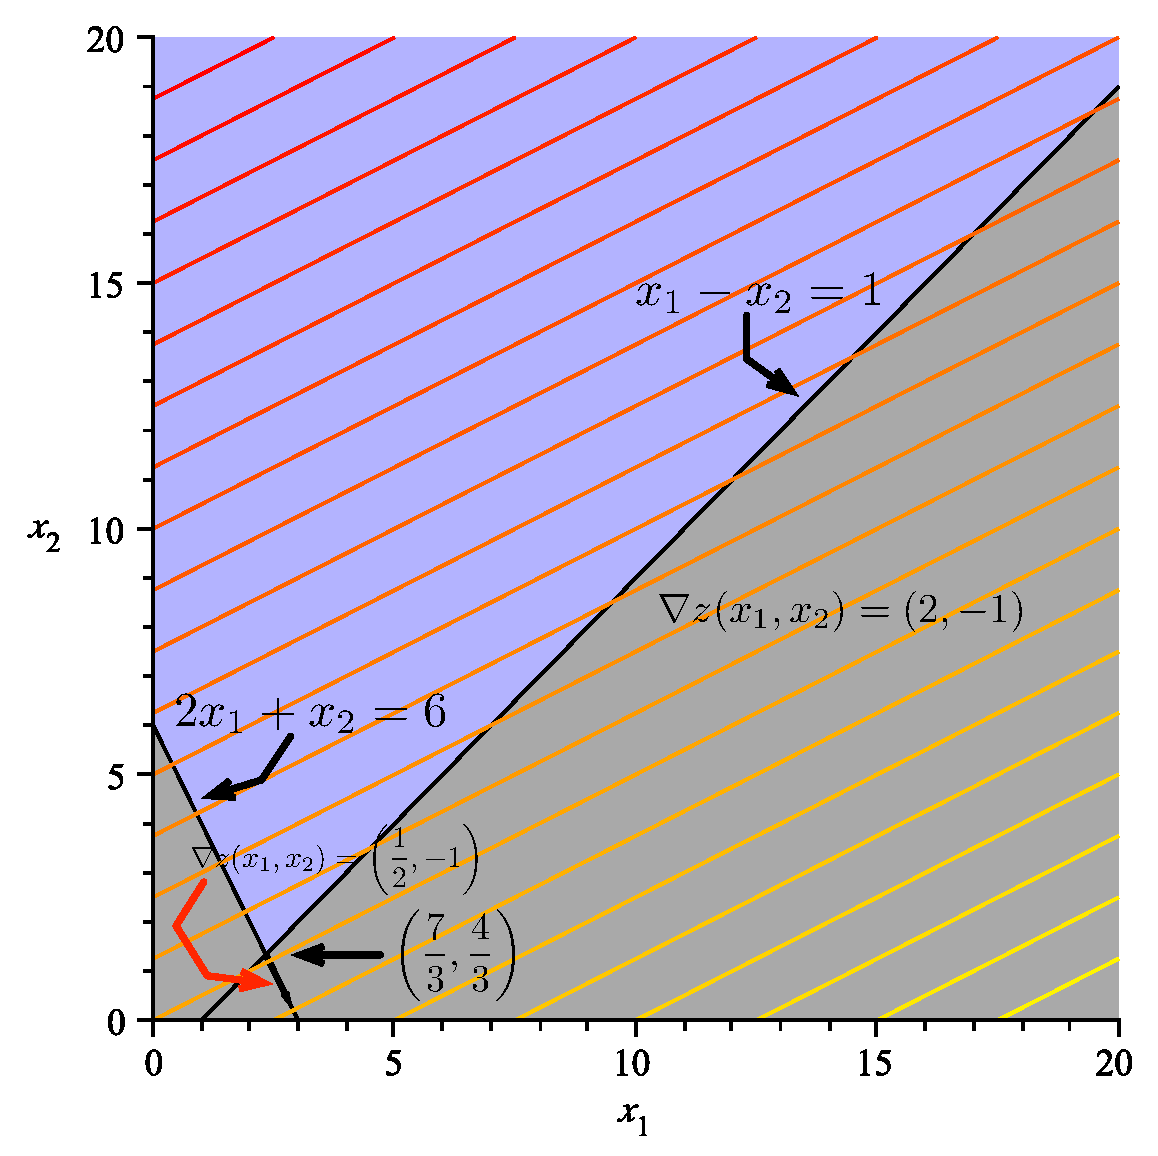
\includegraphics[scale=0.4]{UnboundedFeasibleRegionFiniteSolution.pdf}
\caption{A Linear Programming Problem with Unbounded Feasible Region and Finite Solution: In this problem, the level curves of $z(x_1,x_2)$ increase in a more ``southernly'' direction that in Example \ref{ex:LPUnboundFeasibleRegion2}--that is, \textit{away} from the direction in which the feasible region increases without bound. The point in the feasible region with largest $z(x_1,x_2)$ value is $(7/3,4/3)$. Note again, this is a vertex.}
\label{fig:LPUnboundFeasibleRegion2}
\end{figure}
\label{ex:LPUnboundFeasibleRegion2}
\end{example}
Based on these two examples, we can modify our algorithm for graphically solving a two variable linear programming problems to deal with the case when the feasible region is unbounded.
\begin{algorithm}
\caption{Algorithm for Solving a Linear Programming Problem Graphically--Bounded and Unbounded Case}
\label{alg:GraphLPAlmostGeneral}
\begin{center}
\begin{minipage}[t]{\textwidth-1em}
\underline{\textbf{Algorithm for Solving a Two Variable Linear Programming Problem Graphically}}
\begin{enumerate*}
\item Plot the feasible region defined by the constraints.
\item If the feasible region is empty, then no solution exists.
\item If the feasible region is unbounded goto Line 8. Otherwise, Goto Line 4.
\item Plot the level sets of the objective function.
\item For a maximization problem, identify the level set corresponding the greatest (least, for minimization) objective function value that intersects the feasible region. This point will be at a corner. 
\item The point on the corner intersecting the greatest (least) level set is a solution to the linear programming problem. 
\item \textbf{If the level set corresponding to the greatest (least) objective function value is parallel to a side of the polygon boundary next to the corner identified, then there are infinitely many alternative optimal solutions and any point on this side may be chosen as an optimal solution.} 
\item (The feasible region is unbounded): Plot the level sets of the objective function.
\item If the level sets intersect the feasible region at larger and larger (smaller and smaller for a minimization problem), then the problem is unbounded and the solution is $+\infty$ ($-\infty$ for minimization problems). 
\item Otherwise, identify the level set corresponding the greatest (least, for minimization) objective function value that intersects the feasible region. This point will be at a corner. 
\item The point on the corner intersecting the greatest (least) level set is a solution to the linear programming problem. 
\textbf{If the level set corresponding to the greatest (least) objective function value is parallel to a side of the polygon boundary next to the corner identified, then there are infinitely many alternative optimal solutions and any point on this side may be chosen as an optimal solution.} 
\end{enumerate*}
\end{minipage}
\end{center}
\end{algorithm}

\begin{exercise} Does the following problem have a bounded solution? Why?
\begin{equation}
\left\{
\begin{aligned}
\boldsymbol{\min}\;\;& z(x_1,x_2) = 2x_1 - x_2\\
s.t.\;\;& x_1 - x_2 \leq 1\\
& 2x_1 + x_2 \geq 6\\
&x_1,x_2 \geq 0
\end{aligned}
\right.
\end{equation}
[Hint: Use Figure \ref{fig:LPUnboundFeasibleRegion2} and Algorithm \ref{alg:GraphLPAlmostGeneral}.]
\label{exer:BoundedSolutionQuestion}
\end{exercise}

\begin{exercise} Modify the objective function in Example \ref{ex:LPUnboundFeasibleRegion1} or Example \ref{ex:LPUnboundFeasibleRegion2} to produce a problem with an infinite number of solutions. 
\end{exercise}

\begin{exercise} Modify the objective function in Exercise \ref{exer:BoundedSolutionQuestion} to produce a \textbf{minimization} problem that has a finite solution. Draw the feasible region and level curves of the objective to ``prove'' your example works. [Hint: Think about what direction of increase is required for the level sets of $z(x_1,x_2)$ (or find a trick using Exercise \ref{exer:MinForMax}).]
\end{exercise}

